\section{0427}\label{sec:0427}
\begin{questions}
    \question 海报墙由$n$块宽度相同高度不同的木板组成,那么在此海报墙上能够张贴的最大海报面积是多少?
    设木板宽度为$1$,高度为$h_1,h_2, \dots ,h_n$,海报必须整体都粘贴在墙上,并且不能斜贴。

    \begin{figure}[H]
        \centering
        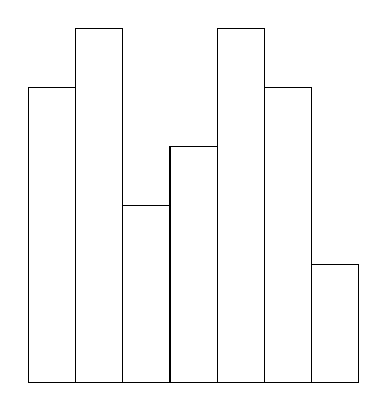
\begin{tikzpicture}[xscale=0.6, yscale=0.75]
            \draw (0,0) rectangle (1,5);
            \draw (1,0) rectangle (2,6);
            \draw (2,0) rectangle (3,3);
            \draw (3,0) rectangle (4,4);
            \draw (4,0) rectangle (5,6);
            \draw (5,0) rectangle (6,5);
            \draw (6,0) rectangle (7,2);
        \end{tikzpicture}
    \end{figure}

    \begin{solution}
        应用扫描线算法,事件点序列为木板高度升序。
        \[
            S(m,n) = \begin{cases}
                \max \begin{cases}
                    (n-m+1) \cdot \min_{m \le i \le n}{h_i}      \\
                    S(m,\mathrm{argmin}_{m \le i \le n}{h_i} -1) \\
                    S(\mathrm{argmin}_{m \le i \le n}{h_i} + 1, n)
                \end{cases} & m < n \\
                h_m                             & m = n \\
                0                               & m > n
            \end{cases}
        \]
        子问题互不重叠,不需要使用动态规划。

        \textbf{伪代码见算法\ref{alg:0427:1}}
    \end{solution}

    \begin{algorithm}[!ht]
        \caption{最大内接矩形}\label{alg:0427:1}
        \begin{algorithmic}[1]
            \Require{$H[1 \dots n]$($n$块木板的高度)}
            \Ensure{$MaxArea$(最大面积)}
            \State $I \gets \Call{SortedList}{H, \mathsf{key=}H[i], \mathsf{value}=i}$
            \Comment{存储的是板子在$H$中的索引,只有顺序查找,用链表}
            \State $MaxArea \gets -1$
            \State $Q \gets \Call{Queue}{\ }$
            \State $\Call{Queue.Push}{Q, (1,n)}$
            \While {$(x,y) \gets \Call{Queue.Pop}{Q}$}
            \If {$y > x$}
            \State $idx \gets \Call{List.findFirst}{I, [x,y]}$ \Comment{找到$[x,y]$区间内最低的板子$idx$}
            \State $area \gets H[idx] \cdot (y-x+1)$ \Comment{算面积}
            \State $MaxArea \gets area$ if $MaxArea < area$
            \State $\Call{Queue.Push}{Q,(x, idx-1)}$ \Comment{添加两个字问题}
            \State $\Call{Queue.Push}{Q,(idx+1, y)}$
            \State $\Call{List.Remove}{I, idx}$   \Comment{移除这块板子}
            \ElsIf {$y = x$}
            \State $area \gets H[x]$ \Comment{算面积}
            \State $MaxArea \gets area$ if $MaxArea < area$
            \State $\Call{List.Remove}{I, x}$   \Comment{移除这块板子}
            \EndIf
            \EndWhile
        \end{algorithmic}
    \end{algorithm}

    \question 平面有两组点,如何证明存在直线可以将这两组点分开?
    \begin{solution}
        \begin{enumerate}
            \item 对两组点分别求凸包,$O(\log n)$
            \item 判断两个凸包是否相交,$O(n)$
        \end{enumerate}
    \end{solution}
\end{questions}
